\title{Vorlesung 8\\Darstellung von Strukturen und semantischen Nachbarschaften in der Wissensbasis}   
%\author[]{Schunkewitsch D.}
%\institute[]{Belarussische Staatliche Universität für Informatik und Radioelektronik}

\begin{frame}
	\titlepage
\end{frame}

\begin{frame}{\\Inhalt der Vorlesung}
	\topline
	\justifying
	Das Konzept der Struktur als eines Fragments der Wissensbasis. Typologie der Strukturen, Rollen der Strukturelemente. Relationen auf Strukturen. Darstellung von Metainformationskonstruktionen in der Wissensbasis. Das Konzept der semantischen Nachbarschaft, Typologie der semantischen Nachbarschaften.
\end{frame}

\begin{frame}{Konzept der Struktur als Fragments der Wissensbasis}
	\topline
	\justifying
	Bei der Ansammlung großer Informationsmengen in einer Wissensbasis wird es notwendig, \textbf{ganze Fragmente} der Wissensbasis zu bestimmen und in der Lage zu sein, sie zu spezifizieren, indem sie als \textbf{separate Entitäten} behandelt werden.
	
	Ein solches Fragment der Wissensbasis wird als Struktur (SC-Struktur) bezeichnet.
	
	Unter \textbf{\textit{Struktur}} verstehen wir eine \textbf{Menge von SC-Elementen}, deren Entfernung zu einer Verletzung der Integrität dieser Menge führen kann.

	Eine Struktur kann sowohl durch explizite Angabe aller Paare des Enthaltenseins von Elementen zu dieser Struktur als auch in Form eines Kreises dargestellt werden, der alle in dieser Struktur vorkommenden Elemente enthält.
\end{frame}

\begin{frame}{Beispiel für die Darstellung einer Struktur als eines Fragments einer Wissensbasis}
	\topline
	\justifying
	\begin{figure}[H]
		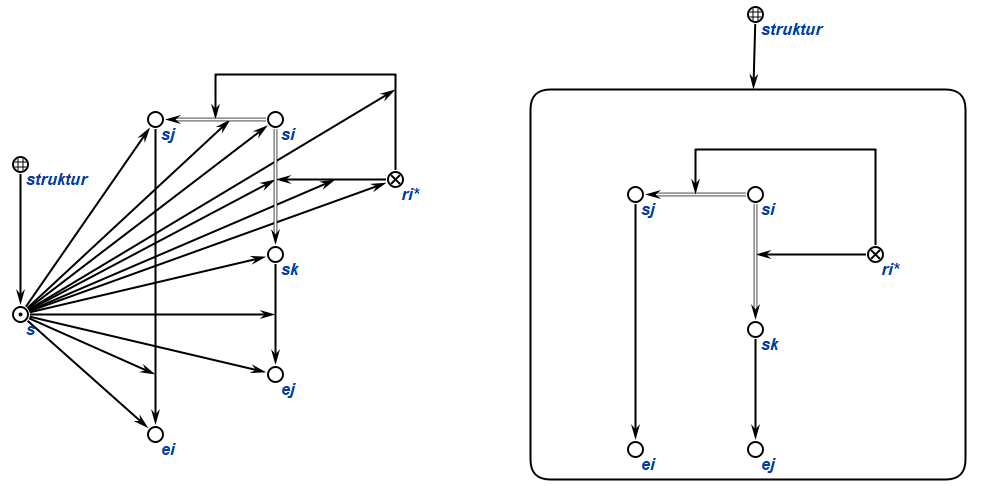
\includegraphics[scale=0.5]{./figures/sd_structures/structure_de.png}
	\end{figure}
\end{frame}

\begin{frame}{\\Typologie der Strukturen}
	\topline
	\justifying
	\begin{SCn}
	\scnheader{Struktur}
	\begin{scnrelfromset}{Unterteilung}
		\scnitem{zusammenhängende Struktur}
		\scnitem{unzusammenhängende Struktur}
	\end{scnrelfromset}
	\begin{scnrelfromset}{Unterteilung}
		\scnitem{triviale Struktur}
		\begin{scnindent}
			\scnidtf{Struktur ohne Verbindungen}
		\end{scnindent}
		\scnitem{nicht-triviale Struktur}
		\begin{scnindent}
			\scnidtf{Struktur, die mindestens eine Verbindung enthält}
		\end{scnindent}
	\end{scnrelfromset}
	\end{SCn}
\end{frame}


\begin{frame}{\\Typologie der Strukturen}
	\topline
	\justifying
	Die im SC-Code dargestellte Struktur entspricht einem Digraphen, dessen Ecken SC-Elemente sind und dessen Bögen Inzidenz-Relationsverbindungen sind, die SC-Konnektoren mit ihren inzidenten SC-Elementen verbinden, die Komponenten der angegebenen SC-Konnektoren sind. Wenn ein auf diese Weise erhaltener Digraph ein zusammenhängender Digraph ist, dann wird die Ausgangsstruktur als eine zusammenhängende Struktur bezeichnet.
	
	Wenn ein auf diese Weise erhaltener Digraph kein zusammenhängender Digraph ist, betrachten wir die Ausgangsstruktur als eine unzusammenhängende Struktur.
\end{frame}


\begin{frame}{\\Typologie der Strukturen}
	\topline
	\justifying
	\vspace{10mm}
	
	Ausgehend von der Stationarität gibt es dynamische Strukturen (Prozesse), deren Zusammensetzung sich im Laufe der Zeit verändert, und statische Strukturen, deren Zusammensetzung sich im Laufe der Zeit nicht verändert.
	
	\begin{SCn}
	\scnheader{Struktur}
	\begin{scnrelfromset}{Unterteilung}
		\scnitem{Prozess}
		\begin{scnindent}
			\scnidtf{dynamische Struktur}
			\scnidtf{nicht-stationäre Struktur}
		\end{scnindent}
		\scnitem{statische Struktur}
		\begin{scnindent}
			\scnidtf{stationäre Struktur}
			\scnidtf{Struktur, die sich im Laufe der Zeit nicht verändert}
		\end{scnindent}
	\end{scnrelfromset}
	\end{SCn}
\end{frame}

\begin{frame}{\\Typologie der Strukturen}
	\topline
	\justifying
	
	Auf der Grundlage der Dauer des Vorhandenseins wird temporale Strukturen und dauerhaft bestehende Strukturen unterschieden.

	\begin{SCn}
	\scnheader{Struktur}
	\begin{scnrelfromset}{Unterteilung}
		\scnitem{temporale Struktur}
		\scnitem{dauerhaft bestehende Struktur}
	\end{scnrelfromset}
	\end{SCn}
\end{frame}

\begin{frame}{\\Rollen der Strukturelemente}
	\topline
	\justifying
	\vspace{10mm}
	
	Zur formalen Darstellung von Strukturen werden Konzepte verwendet, die Rollen von Elementen innerhalb einer Struktur beschreiben. Ein \textbf{\textit{Strukturelement\scnrolesign}} ist ein Nebenkonzept, eine Rollenrelation, die auf alle Elemente jeder Struktur verweist.
	
	\begin{SCn}
	\scnheader{Strukturelement\scnrolesign}
	\begin{scnrelfromset}{Unterteilung}
		\scnitem{unvertretene Menge\scnrolesign}
		\scnitem{vollständig vertretene Menge\scnrolesign}
		\scnitem{teilweise vertretene Menge\scnrolesign}
		\scnitem{Strukturelement, das keine Menge ist\scnrolesign}
	\end{scnrelfromset}
	\end{SCn}
\end{frame}

\begin{frame}{\\Rollen der Strukturelemente}
	\topline
	\justifying
	\vspace{10mm}
	
	\begin{SCn}
	\scnheader{Strukturelement\scnrolesign}
	\begin{scnrelfromset}{Unterteilung}
		\scnitem{maximale Menge\scnrolesign}
		\begin{scnindent}
			\scntext{Erklärung}{Eine Rollenrelation, die eine Struktur mit dem Zeichen einer Menge verbindet, für die es keine Menge gibt, die eine Obermenge der angegebenen Menge wäre und deren Zeichen ein Element derselben Struktur wäre.}
		\end{scnindent}
		\scnitem{nicht-maximale Menge\scnrolesign}
		\begin{scnindent}
			\scntext{Erklärung}{Eine Rollenrelation, die eine Struktur mit einem Zeichen einer Menge verbindet, für die innerhalb dieser Struktur eine Menge existiert, die eine Obermenge der angegebenen Menge ist.}
		\end{scnindent}
	\end{scnrelfromset}
	\end{SCn}
\end{frame}

\begin{frame}{\\Rollen der Strukturelemente}
	\topline
	\justifying
	\vspace{5mm}
	
	\begin{SCn}
	\small
	\scnheader{Strukturelement\scnrolesign}
	\begin{scnrelfromset}{Unterteilung}
		\scnitem{primäres Element\scnrolesign}
		\begin{scnindent}
			\scntext{Erklärung}{Eine Rollenrelation, die auf ein (atomares) Strukturelement verweist, das keine enthaltenen Elemente hat. In diesem Fall kann das entsprechende Paar des Enthaltenseins zwar existieren, aber nicht Teil der gegebenen Struktur sein.}
		\end{scnindent}
		\scnitem{sekundäres Element\scnrolesign}
		\begin{scnindent}
			\scnidtf{Element der gegebenen Struktur mit einer semantischen Ebene von mehr als 2\scnrolesign}
			\scnidtf{nicht-primäres Element\scnrolesign}
			\scntext{Erklärung}{Eine Rollenrelation, die ein Strukturelement angibt und eine Menge von Elementen bezeichnet, von denen notwendigerweise mindestens ein Element der angegebenen Menge Teil der angegebenen Struktur ist.}
		\end{scnindent}
	\end{scnrelfromset}
	\end{SCn}
\end{frame}

\begin{frame}{\\Rollen der Strukturelemente}
	\topline
	\justifying
	
	\scnheader{Strukturelement\scnrolesign}
	\begin{scnrelfromset}{Unterteilung}
		\scnitem{Struktur der ersten Ebene\scnrolesign}
		\begin{scnindent}
			\scntext{Erklärung}{Verbindung von primären Elementen, eine triviale Struktur von primären Elementen oder eine Klasse von primären Elementen}
		\end{scnindent}
		\scnitem{sekundäre Struktur\scnrolesign}
		\begin{scnindent}
			\scntext{Erklärung}{Struktur mit mindestens einem sekundären Element unter ihren Elementen\scnrolesign}
		\end{scnindent}
	\end{scnrelfromset}
\end{frame}

\begin{frame}{\\Beispiel für die Rollen der Strukturelemente}
	\topline
	\justifying
	\begin{figure}[H]
		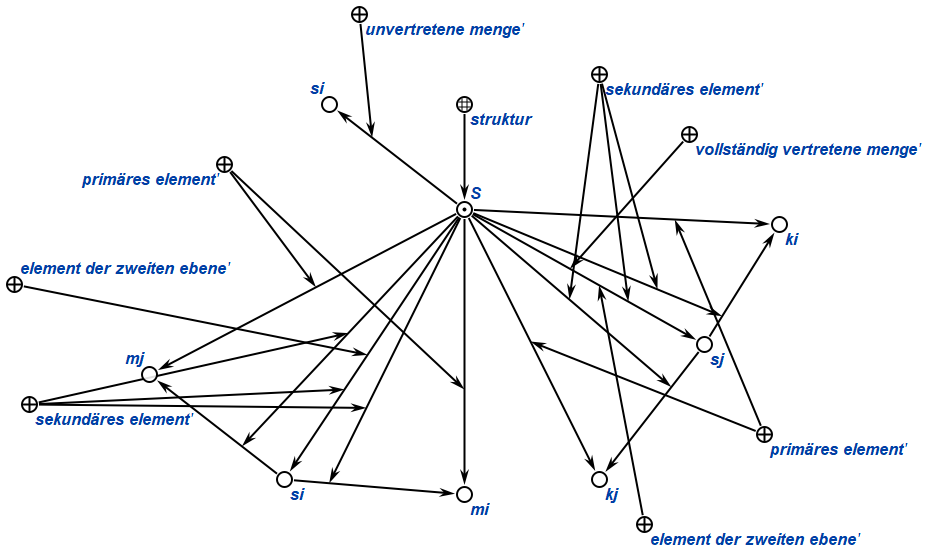
\includegraphics[scale=0.5]{./figures/sd_structures/roles_de.png}
	\end{figure}
\end{frame}

\begin{frame}{\\Relationen auf Strukturen}
	\topline
	\justifying
	\scnheader{binäre Relation*}
	\scnhaselement{Polymorphismus* }
		\begin{scnindent}
			\scnsubset{Anpassung*}
		\end{scnindent}
	\scnhaselement{Polymorphismus*}
	\scnhaselement{Homomorphismus*}
		\begin{scnindent}
		\scnsubset{Anpassung*}
		\end{scnindent}
	\scnhaselement{Homomorphismus*}
	\scnhaselement{Isomorphismus*}
		\begin{scnindent}
		\scnsubset{Anpassung*}
		\end{scnindent}
	\scnhaselement{Isomorphismus*}
	\scnhaselement{Automorphismus*}
		\begin{scnindent}
		\scnsubset{Anpassung*}
		\end{scnindent}
	\scnhaselement{Automorphismus*}
\end{frame}

\begin{frame}{\\Relationen auf Strukturen}
	\topline
	\justifying
	
	\scnheader{Polymorphismus* }
	\scntext{Erklärung}{Polymorphismus* ist eine auf Strukturen festgelegte Anpassung, bei der jedes Element der Anpassungsdefinitionsbereich (erster Struktur) einem oder mehreren Elementen der Anpassungswertebereich (zweiter Struktur) entspricht und es mindestens ein Element der Anpassungsdefinitionsbereich gibt, dem zwei oder mehr Elemente der Anpassungswertebereich entsprechen.}
\end{frame}

\begin{frame}{\\Relationen auf Strukturen}
	\topline
	\justifying
	
	\scnheader{Homomorphismus*}
	\scntext{Erklärung}{Homomorphismus* ist eine auf Strukturen festgelegte Anpassung, bei der jedes Element der Anpassungsdefinitionsbereich (erster Struktur) nur einem Element der Anpassungswertebereich (zweiter Struktur) entspricht.}
\end{frame}

\begin{frame}{\\Relationen auf Strukturen}
	\topline
	\justifying
	
	\scnheader{Isomorphismus*}
	\scntext{Erklärung}{Isomorphismus* ist ein Homomorphismus*, so dass es für jedes Element der Wertebereich genau ein entsprechendes Element der Definitionsbereich gibt}.
	
	
	\scnheader{Automorphismus*}
	\scntext{Erklärung}{Automorphismus* ist ein Isomorphismus*, bei dem die Anpassungsdefinitionsbereich und die Anpassungswertebereich übereinstimmen.}
\end{frame}

\begin{frame}{\\Relationen auf Strukturen}
	\topline
	\justifying
	
	\scnheader{Strukturähnlichkeit*}
	\scnsubset{Anpassung*}
	\scniselement{binäre Relation*}
	\scntext{Erklärung}{Die Strukturähnlichkeit* ist eine Anpassung*, die auf Strukturen festgelegt ist und das Vorhandensein einer Analogie auf Unterstrukturen (Untermengen) der angegebenen Strukturen festlegt. Jedem geordneten Paar, das zur Strukturähnlichkeit* gehört, kann eine Menge von Paaren gegenübergestellt werden, die Ähnlichkeiten* einiger Unterstrukturen und Unterschiede* einiger Unterstrukturen der Ausgangsstrukturen angeben.}
\end{frame}

\begin{frame}{\\Beispiel}
	\topline
	\justifying
	
	\begin{figure}[b]
		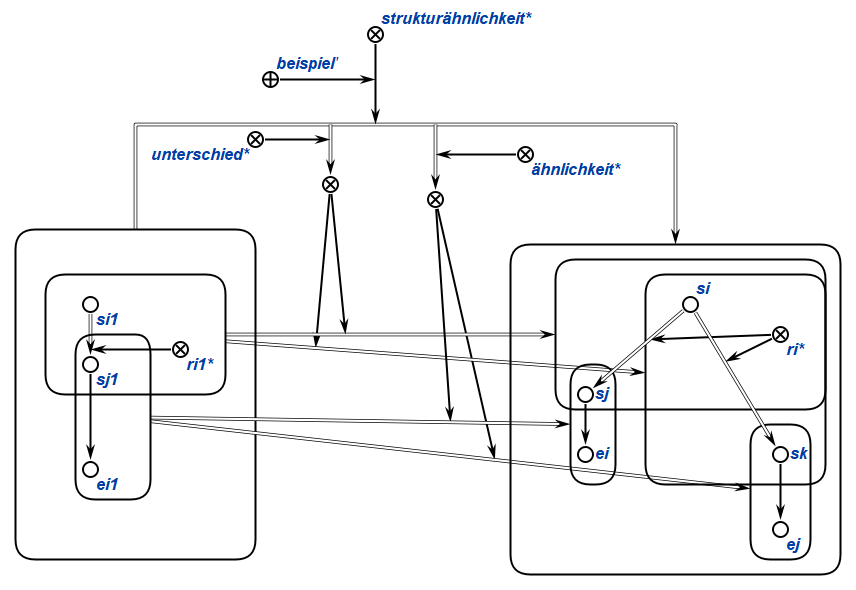
\includegraphics[scale=0.5]{./figures/sd_structures/analogy_de.png}
	\end{figure}
\end{frame}

\begin{frame}{\\Begriff der semantischen Nachbarschaft}
	\topline
	\justifying
	
	\vspace{5mm}
	Für die Spezifikation einzelner Entitäten innerhalb einer Wissensbasis wird das Konzept der \textit{\textbf{semantischen Nachbarschaft}} eingeführt.
	
	Semantische Nachbarschaft ist eine Spezifikation einer bestimmten Entität, deren Zeichen als Schlüsselelement dieser Spezifikation angegeben wird. Im Gegensatz zu anderen Arten von Wissen hat die semantische Nachbarschaft nur ein Schlüsselelement.
	
	Die Menge der Attribute, durch die Entitäten spezifiziert werden können, variiert. Darüber hinaus kann es erforderlich sein, dieselbe Entität unter verschiedenen Aspekten zu spezifizieren und diese Aspekte explizit in der Wissensbasis zu erfassen.
	
	So kann ein und dieselbe Person beispielsweise aus beruflicher, medizinischer, staatsbürgerlicher und anderer Sicht beschrieben werden.
\end{frame}

\begin{frame}{\\Beispiel}
	\topline
	\justifying
	\vspace{10mm}
	
	\begin{figure}[H]
		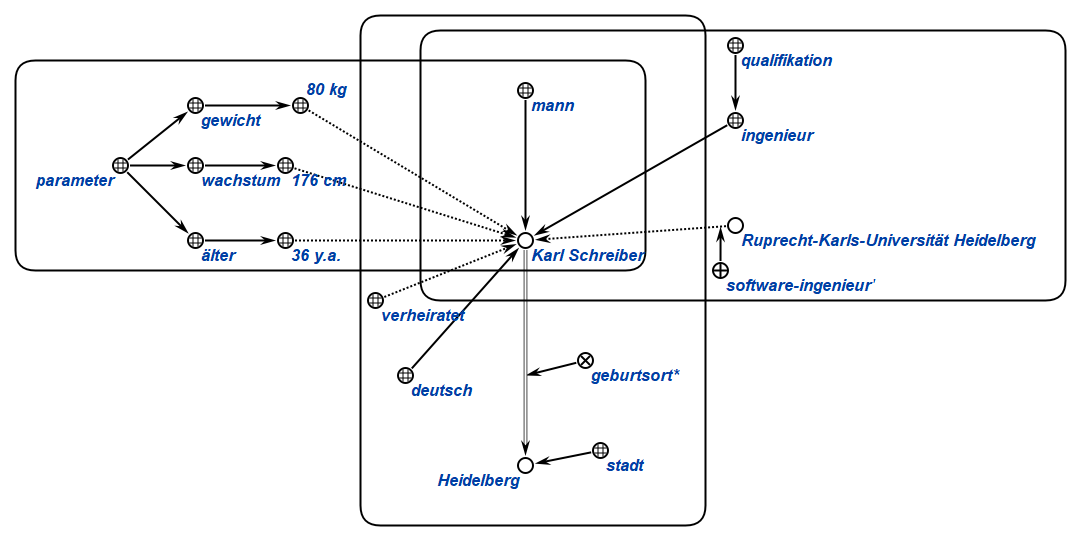
\includegraphics[scale=0.5]{./figures/sd_structures/example_de.png}
	\end{figure}
\end{frame}

\begin{frame}{\\Begriff der semantischen Nachbarschaft}
	\topline
	\justifying
	
	\begin{SCn}
	\scnheader{semantische Nachbarschaft}
	\scnidtf{Beschreibung einer bestimmten Entität, deren Zeichen als Schlüsselelement dieser Spezifikation angegeben ist}
	\scnsubset{Wissen}
	\scnsuperset{semantische Nachbarschaft durch inzidente Konnektoren}
	\scnsuperset{vollständige semantische Nachbarschaft}
	\scnsuperset{grundlegende semantische Nachbarschaft}
	\scnsuperset{spezialisierte semantische Nachbarschaft}
	\end{SCn}

\end{frame}

\begin{frame}{\\Typologie der semantischen Nachbarschaften}
	\topline
	\justifying
	
	\begin{SCn}
	\scnheader{semantische Nachbarschaft durch inzidente Konnektoren}
	\scnsuperset{semantische Nachbarschaft durch ausgehende Bögen}
	\scnsuperset{semantische Nachbarschaft durch eingehende Bögen}
	\scntext{Erklärung}{Die Art der semantischen Nachbarschaft, die alle zu dem angegebenen Element inzidenten Konnektoren umfasst, sowie alle Elemente, die zu den angegebenen Konnektoren inzident sind.}
	\end{SCn}

\end{frame}

\begin{frame}{\\Typologie der semantischen Nachbarschaften}
	\topline
	\justifying
	
	\begin{SCn}
	\scnheader{vollständige semantische Nachbarschaft}
	\scnidtf{vollständige Spezifikation einer beschriebenen Entität}
	
	\scnheader{grundlegende semantische Nachbarschaft}
	\scnidtf{minimale ausreichende semantische Nachbarschaft}
	
	\scnheader{spezialisierte semantische Nachbarschaft}
	\scnidtf{Die Art der semantischen Nachbarschaft, deren Verbindungsmenge für jede Art von Nachbarschaft gesondert angegeben wird.}
	\end{SCn}

\end{frame}

\begin{frame}{\\Typologie der semantischen Nachbarschaften}
	\topline
	\justifying
	
	\begin{SCn}
	\scnheader{spezialisierte semantische Nachbarschaft}
	\scnsuperset{Erklärung}
	\scnsuperset{Anmerkung}
	\scnsuperset{Instanzidentifikationsregel}
	\scnsuperset{terminologische semantische Nachbarschaft}
	\scnsuperset{mengentheoretische semantische Nachbarschaft}
	\scnsuperset{logische semantische Nachbarschaft}
	\scnsuperset{Beschreibung einer typischen Instanz}
	\scnsuperset{Beschreibung der Dekomposition}
	\end{SCn}
	
\end{frame}

